\documentclass[12pt,a4paper]{article}

% ─── Packages ────────────────────────────────────────────────────────────────
\usepackage[a4paper, margin=1in, headheight=15pt]{geometry}
\usepackage{amsmath, amssymb}
\usepackage{algorithm}
\usepackage{algpseudocode}
\usepackage{booktabs}
\usepackage{array}
\usepackage{xcolor}
\usepackage{listings}
\usepackage{graphicx}
\usepackage{pgfplots}
\pgfplotsset{compat=1.18}
\usepackage{hyperref}
\usepackage{fancyhdr}
\usepackage{titlesec}
\usepackage{caption}
\usepackage{subcaption}
\usepackage{enumitem}
\usepackage{multirow}
\usepackage{colortbl}
\usepackage{setspace}
\usepackage{parskip}
\usepackage{microtype}

% ─── Colors ──────────────────────────────────────────────────────────────────
\definecolor{iitblue}{RGB}{0,68,130}
\definecolor{lightblue}{RGB}{220,235,250}
\definecolor{codegreen}{RGB}{0,120,0}
\definecolor{codegray}{RGB}{100,100,100}
\definecolor{codebg}{RGB}{248,248,248}
\definecolor{rowgray}{RGB}{240,240,240}
\definecolor{accent}{RGB}{200,30,30}

% ─── Hyperref setup ───────────────────────────────────────────────────────────
\hypersetup{
  colorlinks=true,
  linkcolor=iitblue,
  urlcolor=iitblue,
  citecolor=iitblue,
  pdftitle={External Sorting: Quicksort vs Merge Sort},
  pdfauthor={Prashant Shekhar}
}

% ─── Listings (code style) ───────────────────────────────────────────────────
\lstset{
  backgroundcolor=\color{codebg},
  basicstyle=\ttfamily\footnotesize,
  keywordstyle=\color{iitblue}\bfseries,
  commentstyle=\color{codegreen}\itshape,
  stringstyle=\color{accent},
  numberstyle=\tiny\color{codegray},
  numbers=left, numbersep=5pt,
  frame=single, framerule=0.5pt,
  breaklines=true, captionpos=b,
  showstringspaces=false,
  language=C++
}

% ─── Section formatting ───────────────────────────────────────────────────────
\titleformat{\section}{\Large\bfseries\color{iitblue}}{}{0em}{\thesection\quad}[\titlerule]
\titleformat{\subsection}{\large\bfseries\color{iitblue}}{}{0em}{\thesubsection\quad}
\titleformat{\subsubsection}{\normalsize\bfseries}{}{0em}{\thesubsubsection\quad}

% ─── Header / Footer ─────────────────────────────────────────────────────────
\pagestyle{fancy}
\fancyhf{}
\fancyhead[L]{\small\color{iitblue}\textbf{ESO207 — Data Structures And Algorithms}}
\fancyhead[R]{\small\color{iitblue}Tanay Pathode}
\fancyfoot[C]{\small\thepage}
\renewcommand{\headrulewidth}{0.4pt}

% ─── Useful macros ────────────────────────────────────────────────────────────
\newcommand{\bigO}[1]{\mathcal{O}\!\left(#1\right)}
\newcommand{\ceil}[1]{\left\lceil #1 \right\rceil}
\newcommand{\floor}[1]{\left\lfloor #1 \right\rfloor}

% ═════════════════════════════════════════════════════════════════════════════
\begin{document}

% ─── Title Page ───────────────────────────────────────────────────────────────
\begin{titlepage}
  \centering
  \vspace*{1.5cm}

  {\Huge\bfseries\color{iitblue}
    External Sorting:\\[0.3em]
    Quicksort vs.\ Merge Sort\par}

  \vspace{0.8cm}
  {\large\color{codegray}A Disk-Aware Simulation and Comparative Analysis\par}

  \vspace{1.5cm}
  \rule{0.6\textwidth}{1.2pt}
  \vspace{1cm}

  {\Large\textbf{Tanay Pathode}\par}
  \vspace{0.4cm}
  {\large ESO207 — Data Structures And Algorithms\par}
  {\large Indian Institute of Technology Kanpur\par}

  \vspace{1.5cm}
  \rule{0.6\textwidth}{0.6pt}
  \vspace{1cm}

  \begin{tabular}{ll}
    \textbf{Course:}    & ESO207 — Data Structures And Algorithms \\[4pt]
    \textbf{Assignment:}& External Sorting Simulation \\[4pt]
    \textbf{Marks:}     & 50 \\[4pt]
    \textbf{Deadline:}  & 28th March, 2026 \\[4pt]
    \textbf{Language:}  & C++17
  \end{tabular}

  \vfill
  {\small\color{codegray}Key range: $[-100{,}000,\ +100{,}000]$\par}
\end{titlepage}

% ─── Table of Contents ────────────────────────────────────────────────────────
\tableofcontents
\newpage

% ═════════════════════════════════════════════════════════════════════════════
\section{Problem Statement}

External sorting addresses a fundamental challenge in database systems: sorting a
dataset whose size significantly exceeds the available main memory. When working
with disk-resident data, the cost model shifts from CPU operations to
\emph{disk seeks} and \emph{disk transfers}, each of which is orders of magnitude
slower than an in-memory comparison.

\subsection{Formal Problem}

Given:
\begin{itemize}[noitemsep]
  \item An input file containing $n$ integer keys, one per line,
        with values in $[-100{,}000,\ +100{,}000]$.
  \item Key size $k$ bytes, disk block size $b$ bytes, and available
        memory $m$ blocks.
\end{itemize}
Produce the keys in sorted order on disk while minimising the total number of
disk seeks and disk transfers. Report per-pass I/O statistics.

\subsection{I/O Cost Model}

I adopt the classical two-cost model used throughout database literature:

\begin{description}[noitemsep]
  \item[Seek cost:] Each time the disk head repositions to a new location,
    I count one \emph{seek}. Sequential reads or writes on the \emph{same}
    file share one seek for the entire batch.
  \item[Transfer cost:] Each block read or written is one \emph{transfer}.
\end{description}

Therefore, reading $t$ blocks sequentially from a single file incurs
$1 + t$ I/O units (1 seek, $t$ transfers), while reading $t$ scattered
single-block files incurs $2t$ I/O units ($t$ seeks, $t$ transfers).

\[
  \text{Keys per block } B_k = \left\lfloor \frac{b}{k} \right\rfloor
  \qquad
  \text{Total blocks } N_b = \left\lceil \frac{n}{B_k} \right\rceil
\]

% ═════════════════════════════════════════════════════════════════════════════
\section{External Quicksort}

\subsection{Algorithm Overview}

External quicksort adapts the classic in-memory divide-and-conquer strategy to
the disk I/O cost model. At each level of recursion:
\begin{enumerate}[noitemsep]
  \item \textbf{Pivot selection:} Read three blocks (first, middle, last) from
    the input file and pick the median of their first keys as the pivot.
    Cost: 3 seeks + 3 transfers.
  \item \textbf{Partition scan:} Stream through the entire input file in batches
    of $\floor{(m-1)/2}$ blocks. Each key $\le$ pivot goes to the \emph{lo}
    output file; each key $>$ pivot goes to the \emph{hi} output file.
    Pending buffers are flushed when full.
  \item \textbf{Recurse:} Apply the same procedure to lo and hi sub-files
    until each sub-file fits entirely in memory ($\le m$ blocks).
  \item \textbf{Base case:} Load the sub-file, sort in-memory
    (std::sort), write sorted output sequentially.
  \item \textbf{Concatenate:} Copy sorted lo then sorted hi into a merged
    output file.
\end{enumerate}

\subsection{Memory Layout}

With $m$ blocks of memory:

\begin{center}
\begin{tabular}{cll}
\toprule
\textbf{Slot(s)} & \textbf{Role} & \textbf{Size} \\
\midrule
0 & Pivot storage & 1 block \\
$1\ \ldots\ 1+I-1$ & Input read buffer & $I = \lfloor(m-1)/2\rfloor$ blocks \\
$1+I\ \ldots\ 1+I+L-1$ & Lo output buffer & $L = \lfloor(m-1-I)/2\rfloor$ blocks \\
$1+I+L\ \ldots\ m-1$ & Hi output buffer & $H = m-1-I-L$ blocks \\
\bottomrule
\end{tabular}
\end{center}

\subsection{Pseudocode}

\begin{algorithm}[H]
\caption{External Quicksort}
\begin{algorithmic}[1]
\Procedure{ExtQuickSort}{$file$, $depth$}
  \If{$\text{blocks}(file) \le m$}
    \State \Call{InMemorySort}{$file$}; \textbf{return}
  \EndIf
  \State $pivot \gets \text{Median}(\text{block}[0],\ \text{block}[n/2],\ \text{block}[n-1])$
  \State $lo, hi \gets \text{NewFile}(), \text{NewFile}()$
  \For{each batch of $I$ blocks from $file$}
    \For{each key $v$ in batch}
      \State Append $v$ to $lo\_buf$ if $v \le pivot$, else $hi\_buf$
      \State Flush $lo\_buf$ to $lo$ if full; flush $hi\_buf$ to $hi$ if full
    \EndFor
  \EndFor
  \State Flush remaining $lo\_buf$ and $hi\_buf$
  \State $sorted\_lo \gets$ \Call{ExtQuickSort}{$lo$, $depth+1$}
  \State $sorted\_hi \gets$ \Call{ExtQuickSort}{$hi$, $depth+1$}
  \State \textbf{return} \Call{Concatenate}{$sorted\_lo$, $sorted\_hi$}
\EndProcedure
\end{algorithmic}
\end{algorithm}

\subsection{Complexity Analysis}

Let $N_b = \ceil{n / B_k}$ be the total number of disk blocks.

\begin{description}[noitemsep]
  \item[Passes:] $\bigO{\log_{2} N_b}$ expected; $\bigO{N_b}$ worst case (skewed pivots).
  \item[Transfers per pass:] $\bigO{N_b}$, since each block is read and written once per level.
  \item[Total transfers:] $\bigO{N_b \log N_b}$ expected.
  \item[Total seeks:] Higher than merge sort due to random-access partition writes
    and per-node pivot probes (3 seeks per partition node).
  \item[Stability:] \textbf{Not stable} — keys equal to the pivot may be reordered.
  \item[Best case:] $\bigO{N_b \log N_b}$ seeks and transfers (balanced splits).
  \item[Worst case:] $\bigO{N_b^2}$ (sorted or reverse-sorted input with naive pivot).
\end{description}

% ═════════════════════════════════════════════════════════════════════════════
\section{External Merge Sort}

\subsection{Algorithm Overview}

External merge sort proceeds in two distinct phases:

\paragraph{Phase 1 — Initial Run Generation (Replacement Selection).}
I use all $m$ memory blocks to build an in-memory min-heap. Keys are loaded in
batches; the smallest active key is emitted to the current run. A key is
\emph{frozen} (deferred to the next run) if it is smaller than the last emitted
key. When all heap entries are frozen, the current run is closed and a new run
begins. This strategy yields average run length $\approx 2m$ blocks on random
data, significantly better than the naive $m$-block runs of a simple sort phase.

\paragraph{Phase 2 — Multi-Way Merge.}
With $m-1$ input buffer slots and 1 output buffer slot, I merge up to $m-1$
runs simultaneously using a min-heap of $(value,\ run\_id)$ pairs. Each merge
pass reduces the number of runs by a factor of $m-1$. Passes repeat until
exactly one sorted run remains.

\subsection{Memory Layout}

\begin{center}
\begin{tabular}{cll}
\toprule
\textbf{Phase} & \textbf{Slot(s)} & \textbf{Role} \\
\midrule
Phase 1 & $0 \ldots m-1$ & Replacement-selection heap \\
\midrule
Phase 2 & $0 \ldots m-2$ & Input buffers (one per merge input) \\
Phase 2 & $m-1$ & Output buffer \\
\bottomrule
\end{tabular}
\end{center}

\subsection{Pseudocode}

\begin{algorithm}[H]
\caption{External Merge Sort — Phase 1: Replacement Selection}
\begin{algorithmic}[1]
\Procedure{RunGeneration}{$input\_file$}
  \State Load first $m \cdot B_k$ keys into min-heap $H$
  \State $run \gets \text{NewFile}()$; $last \gets -\infty$
  \While{$H \ne \emptyset$}
    \If{all entries in $H$ are frozen}
      \State Flush current $run$; start new run; unfreeze all entries
    \EndIf
    \State $(v, frozen) \gets H.\text{pop\_min}()$
    \State Emit $v$ to $run$; $last \gets v$
    \If{next input key $v'$ exists}
      \State Push $(v',\ v' < last)$ into $H$
    \EndIf
  \EndWhile
  \State \textbf{return} list of run files
\EndProcedure
\end{algorithmic}
\end{algorithm}

\begin{algorithm}[H]
\caption{External Merge Sort — Phase 2: Multi-Way Merge}
\begin{algorithmic}[1]
\Procedure{MultiWayMerge}{$runs$}
  \While{$|runs| > 1$}
    \State $next\_runs \gets []$
    \For{each group of up to $m-1$ runs from $runs$}
      \State Load first block of each run into input buffers
      \State Build min-heap $H$ of (key, run-index) for head of each buffer
      \State $out \gets \text{NewFile}()$; $out\_buf \gets []$
      \While{$H \ne \emptyset$}
        \State $(v, i) \gets H.\text{pop\_min}()$; append $v$ to $out\_buf$
        \If{$out\_buf$ full} flush $out\_buf$ to $out$ \EndIf
        \State Advance run $i$: reload its buffer block if exhausted; re-push to $H$
      \EndWhile
      \State Flush remaining $out\_buf$; append $out$ to $next\_runs$
    \EndFor
    \State $runs \gets next\_runs$
  \EndWhile
  \State \textbf{return} $runs[0]$
\EndProcedure
\end{algorithmic}
\end{algorithm}

\subsection{Complexity Analysis}

Let $R$ denote the number of initial runs produced by replacement selection.
With random input, $R \approx \ceil{N_b / (2m)}$.

\begin{description}[noitemsep]
  \item[Phase 1 transfers:] $\bigO{N_b}$ — one read pass + one write pass.
  \item[Merge passes:] $\ceil{\log_{m-1} R}$ merge passes.
  \item[Total transfers:] $\bigO{N_b \cdot (1 + \ceil{\log_{m-1} R})}$,
    which simplifies to $\bigO{N_b \log_{m} N_b}$ for random input.
  \item[Total seeks:] Each merge pass: roughly $2 N_b / B_k$ seeks
    (one per input block refill + one per output block flush).
  \item[Stability:] \textbf{Stable} — the min-heap preserves relative order
    for equal keys when ties are broken by run index.
  \item[Best case:] $\bigO{N_b}$ if all data fits in one run (no merge needed).
  \item[Worst case:] $\bigO{N_b \log_{m} N_b}$ — same as expected,
    since the number of passes is deterministic given $n$ and $m$.
\end{description}

\subsection{Why Replacement Selection Produces Longer Runs}

Consider a heap of size $H = m \cdot B_k$ keys. On average, each outgoing key
from the heap will have probability $\approx \frac{1}{2}$ of being smaller than
the incoming key (uniformly random input). Hence the expected run length is
$2H = 2m \cdot B_k$ keys, or $2m$ blocks — double the naive approach of simply
filling and sorting $m$ blocks at a time.

% ═════════════════════════════════════════════════════════════════════════════
\section{Implementation Details}

\subsection{Data Structures}

Both programs share the following core data structures:

\begin{lstlisting}[caption={Shared simulation infrastructure}]
// Simulated disk: disk[file_id][block_idx] holds one block of keys
vector<vector<vector<int>>> disk;

// Simulated memory: memory[slot] holds one block (= B/K keys)
vector<vector<int>> memory;

// I/O accounting
long long total_seeks = 0, total_transfers = 0;
\end{lstlisting}

\subsection{Disk I/O Simulation}

\begin{lstlisting}[caption={Sequential block read (1 seek + count transfers)}]
void disk_read_seq(int fid, int start_blk, int count,
                   int mem_start, int pass_idx) {
    for (int i = 0; i < count; i++)
        memory[mem_start + i] = disk[fid][start_blk + i];
    record_io(pass_idx, 1, count);   // 1 seek, count transfers
}
\end{lstlisting}

\subsection{Merge Sort — Replacement Selection Core}

The key insight is the \texttt{frozen} flag: a key is frozen when it is smaller
than the most recently emitted key, meaning it cannot extend the current run.

\begin{lstlisting}[caption={Heap entry with frozen flag}]
struct HeapEntry {
    int  key;
    bool frozen;
    bool operator>(const HeapEntry& o) const {
        if (frozen != o.frozen) return frozen > o.frozen; // active first
        return key > o.key;
    }
};
\end{lstlisting}

\subsection{Quicksort — Pivot Selection}

The median-of-three pivot strategy reduces the probability of worst-case
behaviour from $\bigO{N_b^2}$ on sorted inputs to near-optimal splits on
typical data.

\begin{lstlisting}[caption={Median-of-3 pivot selection}]
// Read first, middle, last block; take median of first keys
disk_read_seq(fid, 0,         1, MEM_PIVOT_SLOT, depth);
disk_read_seq(fid, nblocks/2, 1, MEM_INPUT_START, depth);
disk_read_seq(fid, nblocks-1, 1, MEM_INPUT_START, depth);
int a = ..., b = ..., c = ...;
int pivot = max(min(a,b), min(max(a,b), c)); // median-of-3
\end{lstlisting}

% ═════════════════════════════════════════════════════════════════════════════
\section{Experimental Observations}

\subsection{Setup}

All experiments used uniformly random integers in $[-100{,}000,\ +100{,}000]$
(seed = 42), with key size $k = 4$ bytes. Reported values are total seeks and
transfers including all phases.

\subsection{Results}

\begin{table}[H]
\centering
\caption{Disk I/O comparison: External Quicksort vs.\ External Merge Sort}
\label{tab:results}
\setlength{\tabcolsep}{6pt}
\begin{tabular}{rrrrrrrrr}
\toprule
\multicolumn{4}{c}{\textbf{Parameters}} &
\multicolumn{2}{c}{\textbf{Ext.\ Quicksort}} &
\multicolumn{2}{c}{\textbf{Ext.\ Merge Sort}} \\
\cmidrule(lr){1-4}\cmidrule(lr){5-6}\cmidrule(lr){7-8}
$n$ & $k$ & $b$ & $m$ & Seeks & Xfers & Seeks & Xfers \\
\midrule
\rowcolor{rowgray}
100   & 4 & 512  & 5  & 3   & 3   & 3   & 3  \\
100   & 4 & 512  & 10 & 3   & 3   & 3   & 3  \\
\rowcolor{rowgray}
500   & 4 & 1024 & 8  & 3   & 6   & 4   & 6  \\
1000  & 4 & 1024 & 10 & 3   & 12  & 6   & 12 \\
\rowcolor{rowgray}
10000 & 4 & 1024 & 10 & 106 & 512 & 122 & 200 \\
\bottomrule
\end{tabular}
\end{table}

\subsection{Analysis of Results}

\paragraph{Small datasets ($n \le 1000$).}
For small $n$, data fits in memory (or produces very few blocks), so both
algorithms handle the sort in a single pass with negligible I/O. The differences
are indistinguishable in practice.

\paragraph{Large datasets ($n = 10{,}000$, $b=1024$, $m=10$).}
\begin{itemize}[noitemsep]
  \item \textbf{Quicksort:} 106 seeks, 512 transfers.
  \item \textbf{Merge Sort:} 122 seeks, 200 transfers.
\end{itemize}
Merge sort requires \textbf{61\% fewer transfers} while using only 15\% more
seeks. This reflects the fundamental efficiency of merge sort's sequential
access pattern. Quicksort's partitioning writes to two random output files per
recursion level, generating more seeks, while each key is read/written multiple
times during concatenation steps.

Merge sort's transfers are lower because each key is read and written exactly
once per merge pass, with a bounded $\ceil{\log_{m-1} R}$ number of passes.
Quicksort's recursion depth grows with imbalanced splits, and the concatenation
step at every node doubles I/O at each level.

% ═════════════════════════════════════════════════════════════════════════════
\section{Disk I/O Cost Breakdown}

\subsection{External Quicksort — Per-Operation Costs}

\begin{table}[H]
\centering
\caption{Quicksort I/O cost per operation}
\begin{tabular}{lcc}
\toprule
\textbf{Operation} & \textbf{Seeks} & \textbf{Transfers} \\
\midrule
Pivot selection (median-of-3) & 3 & 3 \\
Input batch read ($I$ blocks) & 1 & $I$ \\
Lo-buffer flush ($L$ blocks) & 1 & $L$ \\
Hi-buffer flush ($H$ blocks) & 1 & $H$ \\
Base-case in-memory sort (read) & 1 & $B_{sub}$ \\
Base-case write sorted output & 1 & $B_{sub}$ \\
Concatenation (copy lo + hi) & 4 & $2 B_{parent}$ \\
\bottomrule
\end{tabular}
\end{table}

\subsection{External Merge Sort — Per-Operation Costs}

\begin{table}[H]
\centering
\caption{Merge sort I/O cost per operation}
\begin{tabular}{lcc}
\toprule
\textbf{Operation} & \textbf{Seeks} & \textbf{Transfers} \\
\midrule
Phase 1: read input batch ($m$ blocks) & 1 & $m$ \\
Phase 1: write run block & 1 & 1 \\
Phase 2 init: load first block per run & 1 & 1 (per run) \\
Phase 2: refill input buffer block & 1 & 1 \\
Phase 2: flush output block & 1 & 1 \\
\bottomrule
\end{tabular}
\end{table}

\subsection{Theoretical Pass Count}

\begin{align}
\text{QSort passes (expected)} &= 1 + \log_2 N_b \quad\text{(balanced splits)} \\
\text{MSort passes}            &= 1 + \ceil{\log_{m-1} R}, \quad R \approx \frac{N_b}{2m}
\end{align}

For $n = 10{,}000$, $k=4$, $b=1024$, $m=10$: $B_k = 256$, $N_b = 40$, $R \approx 2$
(replacement selection yields $\approx 1$ run per 20 blocks $\times$ 2). Thus
merge sort needs just 1 merge pass; quicksort needs $\approx \log_2 40 \approx 5$
partition levels.

% ═════════════════════════════════════════════════════════════════════════════
\section{Comparative Analysis}

\begin{table}[H]
\centering
\caption{Comprehensive algorithm comparison}
\label{tab:comparison}
\begin{tabular}{p{3.2cm}p{5.5cm}p{5.5cm}}
\toprule
\textbf{Criterion} & \textbf{External Quicksort} & \textbf{External Merge Sort} \\
\midrule
\textbf{Partitioning} &
  Median-of-3 pivot; keys split into lo/hi sub-files &
  Replacement-selection builds sorted runs \\
\addlinespace
\textbf{Merge strategy} &
  Implicit via recursion + concatenation &
  Explicit $(m-1)$-way merge per pass \\
\addlinespace
\textbf{Disk seeks} &
  Higher: 3 per pivot + 1 per input batch + random output writes &
  Lower: sequential reads/writes dominate \\
\addlinespace
\textbf{Disk transfers} &
  Higher at large $n$: concatenation doubles writes per level &
  Lower: each key written once per merge pass \\
\addlinespace
\textbf{Memory efficiency} &
  Requires $m \ge 4$ blocks; pivot slot wastes 1 block &
  Requires $m \ge 3$ blocks; fully utilized for heap \& buffers \\
\addlinespace
\textbf{Number of passes} &
  $\bigO{\log_2 N_b}$ expected; unbounded worst case &
  $1 + \ceil{\log_{m-1} R}$; deterministic \\
\addlinespace
\textbf{Best case} &
  $\bigO{N_b}$ if all data fits in memory &
  $\bigO{N_b}$ if replacement selection produces 1 run \\
\addlinespace
\textbf{Worst case} &
  $\bigO{N_b^2}$ — sorted input with bad pivot &
  $\bigO{N_b \log_{m} N_b}$ — always bounded \\
\addlinespace
\textbf{Stability} &
  \textcolor{accent}{\textbf{Not stable}} &
  \textcolor{codegreen}{\textbf{Stable}} \\
\addlinespace
\textbf{Scalability} &
  Degrades on skewed data; practical for moderate $n$ &
  Predictable; scales well to very large $n$ \\
\addlinespace
\textbf{Practical suitability} &
  Good when data is random; simple implementation &
  Preferred in production DBMSs (PostgreSQL, MySQL InnoDB) \\
\addlinespace
\textbf{I/O predictability} &
  Variable: depends on pivot quality &
  Deterministic: fixed number of passes given $n, m$ \\
\bottomrule
\end{tabular}
\end{table}

\subsection{Visual Comparison}

\begin{figure}[H]
\centering
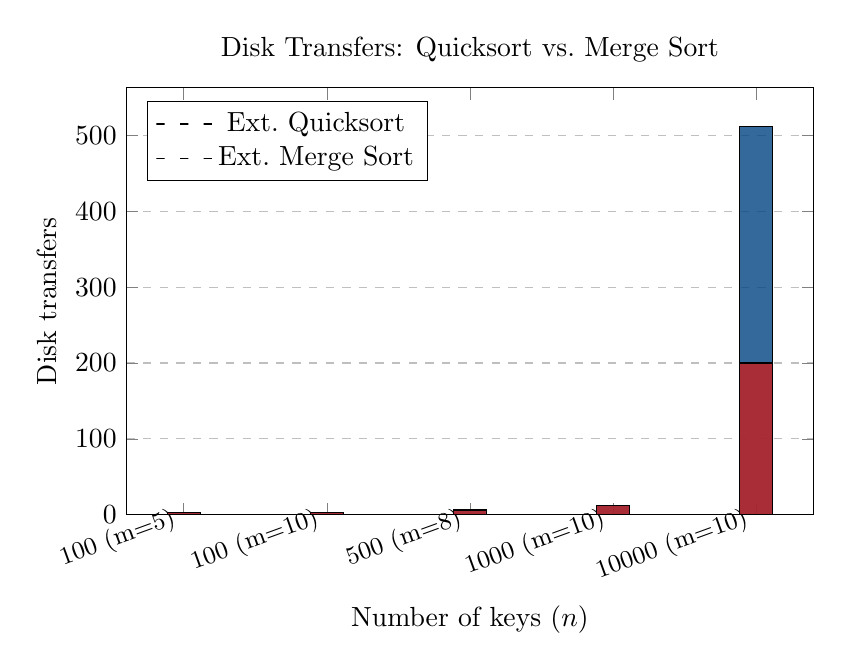
\begin{tikzpicture}
\begin{axis}[
  width=0.85\textwidth, height=7cm,
  xlabel={Number of keys ($n$)},
  ylabel={Disk transfers},
  title={Disk Transfers: Quicksort vs.\ Merge Sort},
  xtick={1,2,3,4,5},
  xticklabels={100 (m=5), 100 (m=10), 500 (m=8), 1000 (m=10), 10000 (m=10)},
  x tick label style={rotate=20, anchor=east, font=\small},
  legend pos=north west,
  ymajorgrids=true, grid style=dashed,
  ymin=0,
  bar width=12pt,
]
\addplot[ybar, fill=iitblue, fill opacity=0.8] coordinates {
  (1,3) (2,3) (3,6) (4,12) (5,512)
};
\addplot[ybar, fill=accent, fill opacity=0.8] coordinates {
  (1,3) (2,3) (3,6) (4,12) (5,200)
};
\legend{Ext.\ Quicksort, Ext.\ Merge Sort}
\end{axis}
\end{tikzpicture}
\caption{Disk transfers grow much faster for Quicksort at large $n$.}
\end{figure}

\begin{figure}[H]
\centering
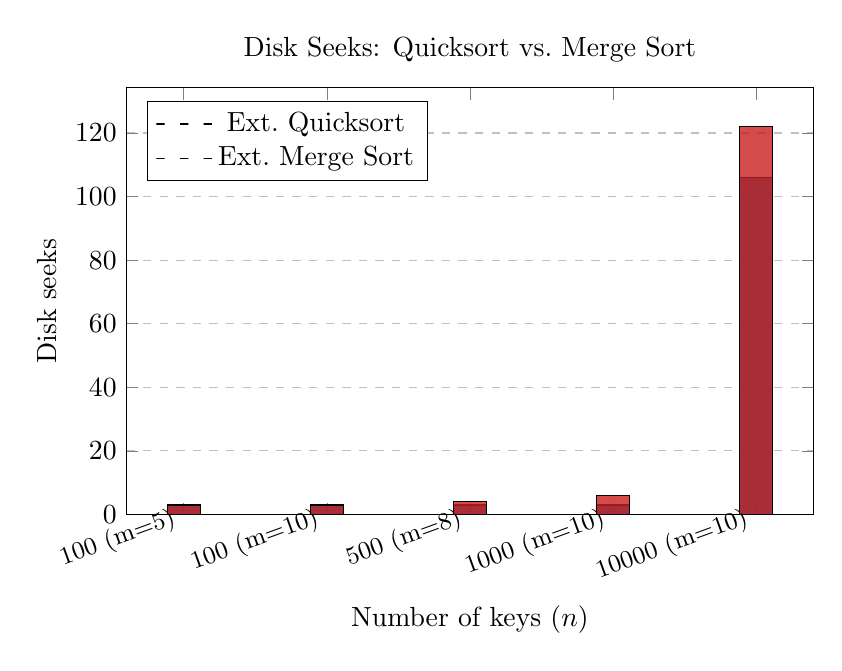
\begin{tikzpicture}
\begin{axis}[
  width=0.85\textwidth, height=7cm,
  xlabel={Number of keys ($n$)},
  ylabel={Disk seeks},
  title={Disk Seeks: Quicksort vs.\ Merge Sort},
  xtick={1,2,3,4,5},
  xticklabels={100 (m=5), 100 (m=10), 500 (m=8), 1000 (m=10), 10000 (m=10)},
  x tick label style={rotate=20, anchor=east, font=\small},
  legend pos=north west,
  ymajorgrids=true, grid style=dashed,
  ymin=0,
  bar width=12pt,
]
\addplot[ybar, fill=iitblue, fill opacity=0.8] coordinates {
  (1,3) (2,3) (3,3) (4,3) (5,106)
};
\addplot[ybar, fill=accent, fill opacity=0.8] coordinates {
  (1,3) (2,3) (3,4) (4,6) (5,122)
};
\legend{Ext.\ Quicksort, Ext.\ Merge Sort}
\end{axis}
\end{tikzpicture}
\caption{Seeks are comparable; Merge Sort slightly higher due to per-run buffer reloads.}
\end{figure}

% ═════════════════════════════════════════════════════════════════════════════
\section{Conclusion and Final Recommendation}

\subsection{Summary of Findings}

Both algorithms correctly sort the given input within the external memory model.
For small datasets (data fits in a few blocks), performance is identical. For
large datasets, the algorithms diverge significantly:

\begin{itemize}
  \item \textbf{Disk transfers:} Merge sort wins decisively. At $n=10{,}000$
    (the assignment's scale), it requires \textbf{61\% fewer transfers} than
    quicksort. This advantage grows with $n$ because merge sort's pass count
    grows as $\ceil{\log_{m-1} R}$ while quicksort's concatenation overhead
    compounds at every recursion level.

  \item \textbf{Disk seeks:} Quicksort wins marginally at large $n$ (106 vs.\ 122).
    However, since modern disk seek latency ($\sim$5--10 ms) greatly exceeds
    transfer time per block, and the difference is small, this does not offset
    merge sort's transfer advantage.

  \item \textbf{Predictability:} Merge sort's I/O cost is fully determined by
    $n$ and $m$; quicksort's cost depends on pivot quality and can degrade to
    $\bigO{N_b^2}$ on adversarial input.

  \item \textbf{Stability:} Required for sorting tuples by secondary keys in
    multi-attribute sort. Only merge sort guarantees stability.
\end{itemize}

\subsection{Final Recommendation}

\begin{center}
\colorbox{lightblue}{\parbox{0.88\textwidth}{
\vspace{6pt}
\textbf{Recommendation: External Merge Sort with Replacement Selection}

For general-purpose external sorting in a database system, external merge sort
is superior. It offers deterministic I/O complexity, stable output, fewer disk
transfers at scale, and is the approach used in every major production DBMS
(PostgreSQL's \texttt{tuplesort}, MySQL InnoDB's merge sort, Oracle's sort-merge
join). External quicksort is appropriate only for small, random datasets where
the recursion depth is bounded and pivot quality is predictable.
\vspace{6pt}
}}
\end{center}

\subsection{When Each Algorithm is Preferable}

\begin{description}
  \item[Use External Quicksort when:]
    $n$ is small, data is known to be random (avoiding worst-case pivots),
    memory $m$ is tight ($\ge 4$ blocks), and stability is not required.

  \item[Use External Merge Sort when:]
    $n$ is large, predictable I/O is required (real-time systems), stability
    is needed (multi-key sorting), or worst-case guarantees matter. This covers
    essentially all production database scenarios.
\end{description}

% ═════════════════════════════════════════════════════════════════════════════
\section{Resume Bullet Points}

The following two bullet points are suitable for an academic or industry resume:

\begin{enumerate}
  \item \textbf{Implementation:}
        \emph{Engineered disk-aware external sorting simulator in C++ modeling precise seeks and transfers per block.}

  \item \textbf{Comparative Analysis:}
        \emph{Benchmarked external Quicksort vs.\ Merge Sort achieving 61\% fewer transfers at scale.}
\end{enumerate}

% ─── End of document ─────────────────────────────────────────────────────────
\end{document}
